% !TeX root = ТеорияОтображений.tex
\section{Операции с множествами}
В прошлом разделе мы рассмотрели как задать множества через свойства, такой способ удобен, но может легко приводить к ошибкам, если не хуже. Рассмотрим пример наивного отношения к множествам, а именно парадокс Рассела. Я приведу две формулировки, школьную версию и строго математическую.

Школьная версия носит название парадокс списков. Положим мы хотим составить список всех книг, которые не содержат в своем тексте своего названия. Нужно ли в этот список вписать его название? Если да, то он будет нарушать свое же условие, если нет, то его придется вписать.

Теперь приведем математическую формулировку. Рассмотрим множество \[M=\{A\mid \varnothing \subset A\}\text{ -- множество множеств, вкючающих в себя пустое.}\]
Под условие подходит любое множество (см. 1.2.2), то есть для всякого множества $D$, $D \in M$. В результате получается так называемое множество всех множеств, теперь покажем к каким последствиям это приведет. Пусть 
\[K=\{F\in M\mid F \notin F\}\text{ -- множество множеств, не содержащих себя.}\]
\begin{commentary}
Если кому-то психологически тяжело воспринимать утверждения $B\in B$ и $B\notin B$, то воспринимайте это как книгу, цитирующую саму себя.
\end{commentary}
Верно ли что $K\in K$? Докажем от противного, предположим $K\notin K$, это попадает под условие множества $K\Rightarrow K\in K$. Противоречие, значит $K\in K$.\\
Но подождите, давайте теперь докажем что $K\notin K$, так же от противного. Положим противное, то есть $K\in K$, тогда условие $K$ не выполнено, ведь в $K$ лежат множества, \textbf{не} содержащие себя $\Rightarrow K\notin K$. Получается противоричивая ситуация, $K\in K$ и $K\notin K$, а такое невозможно.

В чем же проблема? Множество $M$ задано не корректно, в нем даже косвенно не указано откуда нужно брать элементы. Проще говоря наша аксиоматика не допускает существования множества всех множеств.

Обсудим операции с множествами. Для двух множеств $A$ и $B$ мы хотим иметь возможность объединить вместе все их элементы и собрать из них новое множество:
\[A\cup B := \{x\mid x\in A \text{ или } x\in B\}\text{ -- объединение}\]
Далее мы хотим уметь отобрать общие элементы для этих двух множеств, т.е. те, где они пересекаются:
\[A\cap B := \{x\mid x\in A \text{ и } x\in B\}\text{ -- пересечение}\]
А так же элементы, которые есть в первом, но не втором множестве:
\[A\setminus B := \{x\mid x\in A \text{ и } x\notin B\}\text{ -- вычитание}\]
Обратите внимание, что первые две операции симметричны, а третья -- нет. Эти операции удобно визуализировать диаграммами Венна, они интуитивно понятны и не требуют пояснений.
\begin{center}
\begin{venndiagram2sets}[showframe={false}]
\fillA \fillB
\end{venndiagram2sets}
\begin{venndiagram2sets}[showframe={false}]
\fillACapB
\end{venndiagram2sets}
\begin{venndiagram2sets}[showframe={false}]
\fillOnlyA
\end{venndiagram2sets}
\end{center}

Для последней операции нам понадобится новый объект под названием упорядоченная пара, она обозначается как $(p,q)$, где $p$ -- первый элемент, а $q$ -- второй. Мы не будем строго задавать этот объект и ограничемся интуитивным представлением.

Предподожим у нас есть два множества $A=\{0,1,7\}$ и $B=\{g,h\}$, и мы хотим составить таблицу
\begin{wrapfigure}{l}{0.15\textwidth}
\centering
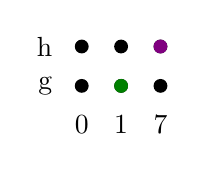
\begin{tikzpicture}[scale=0.5]
% множества
\def\A{0,1,7}
\def\B{g,h}
% координатная сетка
\foreach \x [count=\i] in \A
  \node[below] at (\i,0.5) {\x};
\foreach \y [count=\j] in \B
  \node[left] at (0.5,\j) {\y};
% точки таблицы
\foreach \x [count=\i] in \A
  \foreach \y [count=\j] in \B
    \fill (\i,\j) circle (5pt);
\fill[Green] (2,1) circle (5pt);
\fill[Purple] (3,2) circle (5pt);
\end{tikzpicture}
\end{wrapfigure}
Каждая точка отвечает упорядоченной паре. Например, зеленая точка -- это пара $(1,g)$, фиолетовая -- $(7,h)$. Или можно явно записать таблицу со всеми парами вместо точек:
\[\begin{array}{c|ccc}
h & (0,h) & (1,h) & (7,h) \\
g & (0,g) & (1,g) & (7,g) \\
\hline
 & 0 & 1 & 7 \\
\end{array}\]
Явно множество всех таких пар будет задаваться следующим образом:
\[\{(0,g),(1,g),(7,g),(0,h),(1,h),(7,h)\}\]
Зададим его через свойства, но для этого нужно их сформулировать. Принцип такой, на первых позициях стоят только элементы $A$, а на вторых только элементы $B$.
\begin{definition}\label{def:Dprod}
Декартовым произведением множеств $A$ и $B$ называется множество упорядоченных пар $(p,q)$, со свойством $p\in A$ и $q\in B$.
\[A\times B := \{(p,q)\mid p\in A,q\in B\}\text{ -- декартово произведение}\]
Если $A$ и $B$ -- дискретные множества, то декартово произведение визуализируется через сетку или таблицу.
\end{definition}
\begin{example}
Рассмотрим результаты разных операций на примере $\{1,2\}$ и $\{1,3\}$.
\begin{multicols}{2}
\begin{center}
\noindent
$\{1,2\}\cup \{1,3\}=\{1,2,3\}$ \\
$\{1,2\}\cap \{1,3\}=\{1\}$ \\
$\{1,2\}\setminus \{1,3\}=\{2\}$ \\
$\{1,3\}\setminus \{1,2\}=\{3\}$
\end{center}
\columnbreak
\begin{center}
\noindent
\ \\
$\{1,2\}\times \{1,3\}=\{(1,1),(1,3),(2,1),(2,3)\}$\\
$\{1,3\}\times \{1,2\}=\{(1,1),(1,2),(3,1),(3,2)\}$
\end{center}
\end{multicols}
Здесь видно что вычитание и декартово произведение не симметричны, если поменять множества местами -- результат изменится, как, например, при разности чисел.
\end{example}

\begin{multicols}{2}
\begin{exercise}
\ \\
\noindent\textbf{1.}
Сформулируйте отрицание\\
$x_1\in A\cup B$, 
$x_2\in A\cap B$, 
$x_3\in A\setminus B$.

\medskip\noindent\textbf{2.}
Пусть $A$ и $B$ -- множества.
Докажите,\\ что $A\setminus A=\varnothing,\ (A\setminus B)\cup B=A,$

\medskip\noindent\textbf{3.}
Задайте явно и визуализируйте\\
$\{\alpha,\beta,\gamma\}\times\{1,2,3\},\ \{0,1\}^2,\\
\{1,2,3\}\times\{\alpha,\beta,\gamma\},\ \{0,1\}^3$.

\medskip\noindent\textbf{4.}
Задайте через свойства\\
$U$ -- множество четных чисел\\
$S$ -- множество нечетных чисел.

\medskip\noindent\textbf{5.}
Докажите что нет одновременно\\
четных и нечетных чисел\\
т.е. что $U\cap S$ пусто.

\medskip\noindent\textbf{6.}
Докажите что $0\notin S$ и $U\cup S=\mathbb{Z}$.

\medskip\noindent\textbf{7.}
Пусть $X=\{0,3,b,c\},Y=\{0,c\},\\Z=\{3,b,d\}$.
Задайте явно:\\
$\begin{array}{llll}
X\cup Y & X\setminus Z & Z\cup X\cup Y & (Y\cap X)\times Y\\
Y\cup Z & Y\setminus Z & X\cap Y\cap Z & Y\cap (X\times Y)\\
Y\cap Z & (X\setminus Z)\setminus Y & (Y\cup Z)\setminus X & (Y\cup X)\times Y\\
Z\cap X & X\setminus (Z\setminus Y) & Y\cup (Z\setminus X) & Y\cup (X\times Y).
\end{array}$

\medskip\noindent\textbf{8.}
Пусть $A$ и $B$ -- произвольные множества.\\ Докажите\\
$x\in A\Rightarrow x\in A\cup B$\\
$x\in A\cap B\Rightarrow x\in A$\\
Верно ли обратное? Приведите примеры.

\medskip\noindent\textbf{9.}
Схематично визуализируйте следующие множества: 
$\mathbb{N}\times\{0,1\},\{0,1\}\times\mathbb{N},\mathbb{N}^2,\mathbb{N}\times\mathbb{Z}$.
\end{exercise}
\end{multicols}
